\documentclass[11pt, oneside]{article}   	% use "amsart" instead of "article" for AMSLaTeX format
\usepackage{geometry}                		% See geometry.pdf to learn the layout options. There are lots.
\geometry{letterpaper}                   		% ... or a4paper or a5paper or ... 
%\geometry{landscape}                		% Activate for rotated page geometry
%\usepackage[parfill]{parskip}    		% Activate to begin paragraphs with an empty line rather than an indent
\usepackage{graphicx}				% Use pdf, png, jpg, or eps§ with pdflatex; use eps in DVI mode\usepackage{apacite}
\usepackage{apacite}							% TeX will automatically convert eps --> pdf in pdflatex		
\usepackage{amssymb}
\usepackage[acronym]{glossaries}
\makeglossaries
\newacronym{ran}{RAN}{Radio Access Networks}
%SetFonts

%SetFonts
%File mb-bibtex.tex, then \jobname = mb-bibtex
\usepackage{filecontents}        % loading package filecontents
% writing file \jobname.bib, for example mb-bibtex.bib.
\begin{filecontents*}{\jobname.bib}
@book{white2012hadoop,
  title={Hadoop: The definitive guide},
  author={White, Tom},
  year={2012},
  publisher={" O'Reilly Media, Inc."}
}
@article{ratti2006mobile,
  title={Mobile landscapes: using location data from cell phones for urban analysis},
  author={Ratti, Carlo and Frenchman, Dennis and Pulselli, Riccardo Maria and Williams, Sarah},
  journal={Environment and Planning B: Planning and Design},
  volume={33},
  number={5},
  pages={727--748},
  year={2006},
  publisher={SAGE Publications}
}
@article{chen2014big,
  title={Big data: a survey},
  author={Chen, Min and Mao, Shiwen and Liu, Yunhao},
  journal={Mobile Networks and Applications},
  volume={19},
  number={2},
  pages={171--209},
  year={2014},
  publisher={Springer}
}
@inproceedings{laurila2012mobile,
  title={The mobile data challenge: Big data for mobile computing research},
  author={Laurila, Juha K and Gatica-Perez, Daniel and Aad, Imad and Bornet, Olivier and Do, Trinh-Minh-Tri and Dousse, Olivier and Eberle, Julien and Miettinen, Markus and others},
  booktitle={Pervasive Computing},
  number={EPFL-CONF-192489},
  year={2012}
}
@inproceedings{agrawal2011big,
  title={Big data and cloud computing: current state and future opportunities},
  author={Agrawal, Divyakant and Das, Sudipto and El Abbadi, Amr},
  booktitle={Proceedings ofthe 14th International Conference on Extending Database Technology},
  pages={530--533},
  year={2011},
  organization={ACM}
}
@article{herrera2010evaluation,
  title={Evaluation of traffic data obtained via GPS-enabled mobile phones: The Mobile Century field experiment},
  author={Herrera, Juan C and Work, Daniel B and Herring, Ryan and Ban, Xuegang Jeff and Jacobson, Quinn and Bayen, Alexandre M},
  journal={Transportation Research Part C: Emerging Technologies},
  volume={18},
  number={4},
  pages={568--583},
  year={2010},
  publisher={Elsevier}
}
@article{rao2003evolution,
  title={Evolution of mobile location-based services},
  author={Rao, Bharat and Minakakis, Louis},
  journal={Communications of the ACM},
  volume={46},
  number={12},
  pages={61--65},
  year={2003},
  publisher={ACM}
}
@book{schiller2004location,
  title={Location-based services},
  author={Schiller, Jochen and Voisard, Agn{\`e}s},
  year={2004},
  publisher={Elsevier}
}
@inproceedings{barkhuus2003location,
  title={Location-Based Services for Mobile Telephony: a Study of Users' Privacy Concerns.},
  author={Barkhuus, Louise and Dey, Anind K},
  booktitle={Interact},
  volume={3},
  pages={702--712},
  year={2003},
  organization={Citeseer}
}	
@article{dean2008mapreduce,
  title={MapReduce: simplified data processing on large clusters},
  author={Dean, Jeffrey and Ghemawat, Sanjay},
  journal={Communications of the ACM},
  volume={51},
  number={1},
  pages={107--113},
  year={2008},
  publisher={ACM}
}
@article{dhar2011challenges,
  title={Challenges and business models for mobile location-based services and advertising},
  author={Dhar, Subhankar and Varshney, Upkar},
  journal={Communications of the ACM},
  volume={54},
  number={5},
  pages={121--128},
  year={2011},
  publisher={ACM}
}
@inproceedings{gruteser2003anonymous,
  title={Anonymous usage of location-based services through spatial and temporal cloaking},
  author={Gruteser, Marco and Grunwald, Dirk},
  booktitle={Proceedings of the 1st international conference on Mobile systems, applications and services},
  pages={31--42},
  year={2003},
  organization={ACM}
}
@inproceedings{tsalgatidou2003mobile,
  title={Mobile E-Commerce and Location-Based Services: Technology and Requirements.},
  author={Tsalgatidou, Aphrodite and Veijalainen, Jari and Markkula, Jouni and Katasonov, Artem and Hadjiefthymiades, Stathes},
  booktitle={ScanGIS},
  pages={1--14},
  year={2003},
  organization={Citeseer}
}	
@inproceedings{bravo2004advanced,
  title={Advanced positioning and location based services in 4G mobile-IP radio access networks},
  author={Bravo, A Montilla and Moreno, Jos{\'e} Ignacio and Soto, Ignacio},
  booktitle={Personal, Indoor and Mobile Radio Communications, 2004. PIMRC 2004. 15th IEEE International Symposium on},
  volume={2},
  pages={1085--1089},
  year={2004},
  organization={IEEE}
}
@inproceedings{chow2006peer,
  title={A peer-to-peer spatial cloaking algorithm for anonymous location-based service},
  author={Chow, Chi-Yin and Mokbel, Mohamed F and Liu, Xuan},
  booktitle={Proceedings of the 14th annual ACM international symposium on Advances in geographic information systems},
  pages={171--178},
  year={2006},
  organization={ACM}
}
@inproceedings{borthakur2011apache,
  title={Apache Hadoop goes realtime at Facebook},
  author={Borthakur, Dhruba and Gray, Jonathan and Sarma, Joydeep Sen and Muthukkaruppan, Kannan and Spiegelberg, Nicolas and Kuang, Hairong and Ranganathan, Karthik and Molkov, Dmytro and Menon, Aravind and Rash, Samuel and others},
  booktitle={Proceedings of the 2011 ACM SIGMOD International Conference on Management of data},
  pages={1071--1080},
  year={2011},
  organization={ACM}
}
@article{manyika2011big,
  title={Big data: The next frontier for innovation, competition, and productivity},
  author={Manyika, James and Chui, Michael and Brown, Brad and Bughin, Jacques and Dobbs, Richard and Roxburgh, Charles and Byers, Angela H},
  year={2011}
}
@article{van2005linking,
  title={Linking perceived value and loyalty in location-based mobile services},
  author={van Riel, Allard CR and Pura, Minna},
  journal={Managing Service Quality: An International Journal},
  volume={15},
  number={6},
  pages={509--538},
  year={2005},
  publisher={Emerald Group Publishing Limited}
}
@inproceedings{shvachko2010hadoop,
  title={The hadoop distributed file system},
  author={Shvachko, Konstantin and Kuang, Hairong and Radia, Sanjay and Chansler, Robert},
  booktitle={2010 IEEE 26th symposium on mass storage systems and technologies (MSST)},
  pages={1--10},
  year={2010},
  organization={IEEE}
}
@article{mehtahadoop,
  title={Hadoop Ecosystem: An Introduction},
  author={Mehta, Sneha and Mehta, Viral}
}

@misc{apachehadoop,
  title = {{Apache\texttrademark Hadoop}},
  howpublished = "\url{http://hadoop.apache.org}",
}

\end{filecontents*}



\title{Big Data Research and Use Cases for Location Based Service using Mobile Radio Access Networks}
\author{Gavin Ni \\Qrious Limited, New Zealand \\gavin.ni@qrious.co.nz}
%\date{}							% Activate to display a given date or no date
\providecommand{\keywords}[1]{\textbf{\textit{Keywords:}} #1}
\begin{document}
\maketitle
\begin{abstract}
  Location-based services (LBS) provide the ability to find the geographical location of a mobile device and then provide services based on that location. Researches in using Location Based Services using Mobile data have been well established \fullcite{}. Most of these researches are discuss the LBS based on Global Positioning System(GPS) enabled mobile devices \fullcite{}, where people often raised concerns on the data privacy \fullcite{} on the personal information level. This paper is to identify the gap that research in LBS between using GPS data and using Radio Access Networks(RAN) data. Furthermore, discuss use cases and future works for Big Data analytics in LBS using RAN data.
\end{abstract}
\keywords{Big Data, Mobile, RAN, LBS}

\section{Introduction}

\subsection{Big Data}
Big Data refers to datasets that grow so large that it is difficult to capture, store, manage, share, analyze and visualize using the typical database software tools \fullcite{}.  Gartner's definition of the 3Vs is still widely used, and in agreement with a consensual definition that states that "Big Data represents the Information assets characterized by such a High Volume, Velocity and Variety to require specific Technology and Analytical Methods for its transformation into Value" \fullcite{}. Typical Big Data sources include Web Data, Event Logs, Censors Data, Social Network Data, Machine Generated etc.

\subsubsection{Characteristics}
\begin{itemize}
\item Huge
\item Distributed Dispersed over many servers 
\item Dynamic Items add/deleted/modified continuously
\item Heterogeneous Many agents access/update data
\item Noisy
\item Inherent
\item Unintentional/Malicious
\item Unstructured/semi-structured
\item No database schema
\item Complex interrelationships
\end{itemize}

\subsubsection{Architecture Framework and Use Cases}
\begin{itemize}
\item Offline Analytics
\item Near Realtime Analytics 
\item Realtime Analytics
\end{itemize}

\begin{figure}
  \centering
  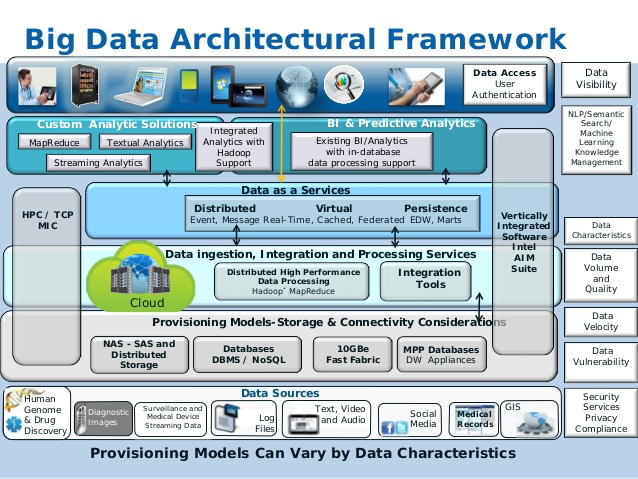
\includegraphics[width=\linewidth]{big-data-solutions.png}
  \caption{Big Data Architecture Framework}
  \label{fig:bigdatasolutions}
\end{figure}



\subsection{Location Based Services}
Based on Localization-Based Systems LBS can be broadly divided:

\textbf{Network-based techniques} utilize the service provider's network infrastructure to identify the location of the handset. The advantage of network-based techniques - from a mobile operator's point of view - is that they can be implemented non-intrusively, without affecting the handsets.

\begin{itemize}
\item 3G Network
\item 4G Network 
\end{itemize}

\textbf{Handset-based technology} requires installing client software on the handset to determine its location. This technique determines the location of the handset by computing its location by cell identification, signal strengths of the home and neighbouring cells, which is continuously sent to the carrier. In addition, if the handset is also equipped with GPS then significantly more precise location information is sent from the handset to the carrier.

By using the SIM in GSM and UMTS handsets, it is possible to obtain raw radio measurements from the handset. The measurements that are available can include the serving Cell ID, round trip time and signal strength. The type of information obtained via the SIM can differ from what is available from the handset. For example, it may not be possible to obtain any raw measurements from the handset directly, yet still obtain measurements via the SIM.

\textbf{Hybrid positioning systems} use a combination of network-based and handset-based technologies for location determination. One example would be some modes of Assisted GPS, which can both use GPS and network information to compute the location. Both types of data are thus used by the telephone to make the location more accurate (i.e. A-GPS). Alternatively tracking with both systems can also occur by having the phone attain his GPS-location directly from the satellites, and then having the information sent via the network to the person that is trying to locate the telephone. Google Latitude, for instance, allows such mobile phone tracking.

\subsubsection{Metrics}
\begin{itemize}
\item Accuracy
\item Reliability
\item Availability
\item Frequency 
\end{itemize}

\section{Related Work}
Apache Hadoop Ecosystem is a framework of various types of complex and evolving tools see Figure \ref{fig:hadoopecosystem}  and components from Apache Foundation which have proficient advantage in solving big Data and Business Intelligence(BI) problems. In \fullcite{mehtahadoop}, the Hadoop tools set had been labeled as Data Management, Data Access, Data Process and Data Storage.

To understand Hadoop Ecosystem and what problem it can solve, in the follow subsections we will explain Hadoop Core system, HDFS and MapReduce, and Hadoop extension tools that make Hadoop core system even powerful and easy of use and maintain. 


\section{Discussion}

\section{Summary and Future Research}

\printglossaries
\bibliographystyle{apacite}
\bibliography{\jobname}
\end{document}  